\section{Results}\label{results}

\subsection{Long Read Alignment Assembler (LRAA) for isoform identification and quantification}\label{long-read-alignment-assembler-lraa-for-isoform-identification-and-quantification}

LRAA was designed as a unified framework for reference-guided and reference-free isoform discovery and quantification from spliced genome alignments of long-read RNA sequencing data. The method explicitly addresses two pervasive challenges in long-read transcriptomics: incomplete transcript coverage that yields partial isoform fragments, and ambiguity in read compatibility across overlapping transcript isoform structures. To resolve these challenges, LRAA integrates splice-graph based structural modeling with probabilistic isoform quantification using expectation maximization (EM), allowing isoform discovery and abundance estimation to be tightly coupled within a single inference framework (\textbf{Fig.~\ref{fig:1}} and \textbf{Supplementary Fig.~\ref{sfig:1}}).

LRAA operates on strand-specific spliced alignments of long reads to the reference genome. For each chromosome and transcriptional orientation, LRAA constructs a splice graph whose nodes represent partitioned exon segments, splice junctions, and transcript boundary features including transcription start sites (TSS) and transcription end sites (TES), typically corresponding to polyadenylation sites. Separate splice graphs are constructed for multi-exonic and single-exon alignments to prevent inappropriate coupling of spliced and unspliced read structures (\textbf{Supplementary Fig.~\ref{sfig:1}}).

Each read alignment is decomposed into its corresponding path through the splice graph and encoded as an ordered sequence of labeled graph elements. Reads that cannot be assigned a compatible splice-graph path are evaluated for transcriptome-based rescue. In this step, candidate failed reads are aligned directly to transcript cDNA sequences, and accepted transcriptome alignments are projected back onto genomic coordinates and converted into splice-graph paths. In reference-guided runs, this rescue procedure allows reads supporting multi-exon annotated transcripts to contribute during guided isoform assembly, improving retention of annotation-supported isoforms whose genome alignments are especially challenging, including cases involving locally repetitive sequences or microexon-containing isoforms.

Read alignments are grouped into read compatibility classes (RCCs), which represent sets of reads that are structurally indistinguishable with respect to exon--intron architecture and transcript boundaries according to paths traversed in the splice graph. This representation provides a compact description of read support while explicitly capturing ambiguity arising from partial transcript coverage and shared exons.

Candidate isoforms are assembled by hierarchically merging transcriptionally compatible RCCs based on shared splice patterns, transcript boundaries, and genomic overlap. Shorter RCCs that are fully contained within multiple longer, mutually splice-incompatible RCCs are treated as shared evidence for those longer candidates rather than as independent isoforms, reflecting partial reads whose observed structure does not distinguish among the longer transcript models. Assembled isoforms are grouped into gene-level components based on shared splice graph structure and overlap thresholds, yielding a set of candidate isoforms and their supporting RCCs.

Isoform abundance estimation is performed independently within each gene-level component using an EM algorithm that fractionally assigns reads from shared RCCs to compatible isoforms based on maximum likelihood. Reads that are uniquely compatible with a single isoform contribute entirely to its abundance estimate, whereas reads compatible with multiple isoforms are probabilistically allocated according to current isoform proportion estimates. To mitigate over-fragmentation of isoform models and suppress low-confidence transcripts, LRAA applies iterative filtering during quantification. Isoforms whose estimated abundance falls below a minimum fraction of corresponding gene expression (default minimum of 1\% presumed biologically relevant) are removed, and remaining isoforms are re-quantified. This process effectively reabsorbs read support from filtered isoforms into remaining compatible models and continues until all retained isoforms exceed the minimum gene-fractional expression threshold.

To further improve robustness under conditions of high read ambiguity, the EM-based quantification incorporates additional modeling constraints informed by long-read sequencing characteristics. These include regularization to stabilize abundance estimates when reads are compatible with multiple isoforms, as well as weighting of ambiguous read assignments based on agreement with transcript 3′ termini, reflecting the increased reliability of read evidence near polyadenylation sites based on 3' poly-A primed cDNA synthesis. This approach prioritizes biologically informative read support while mitigating overconfidence arising from partial or weakly informative alignments.

LRAA supports three execution modes within the same algorithmic framework. In quantification-only mode, isoform discovery is bypassed and reads are assigned directly to a provided reference annotation using EM-based abundance estimation. In reference-guided mode, known transcript structures are incorporated into splice graph construction to guide discovery of additional isoforms while retaining sensitivity to novel transcript variants. In annotation-free (de novo) mode, isoform discovery and quantification rely solely on long-read alignments and the reference genome sequence, without requiring any prior transcript annotation. Across all modes, the same splice-graph representation, read compatibility modeling, and EM-based quantification strategy are used.

\begin{center}
\pandocbounded{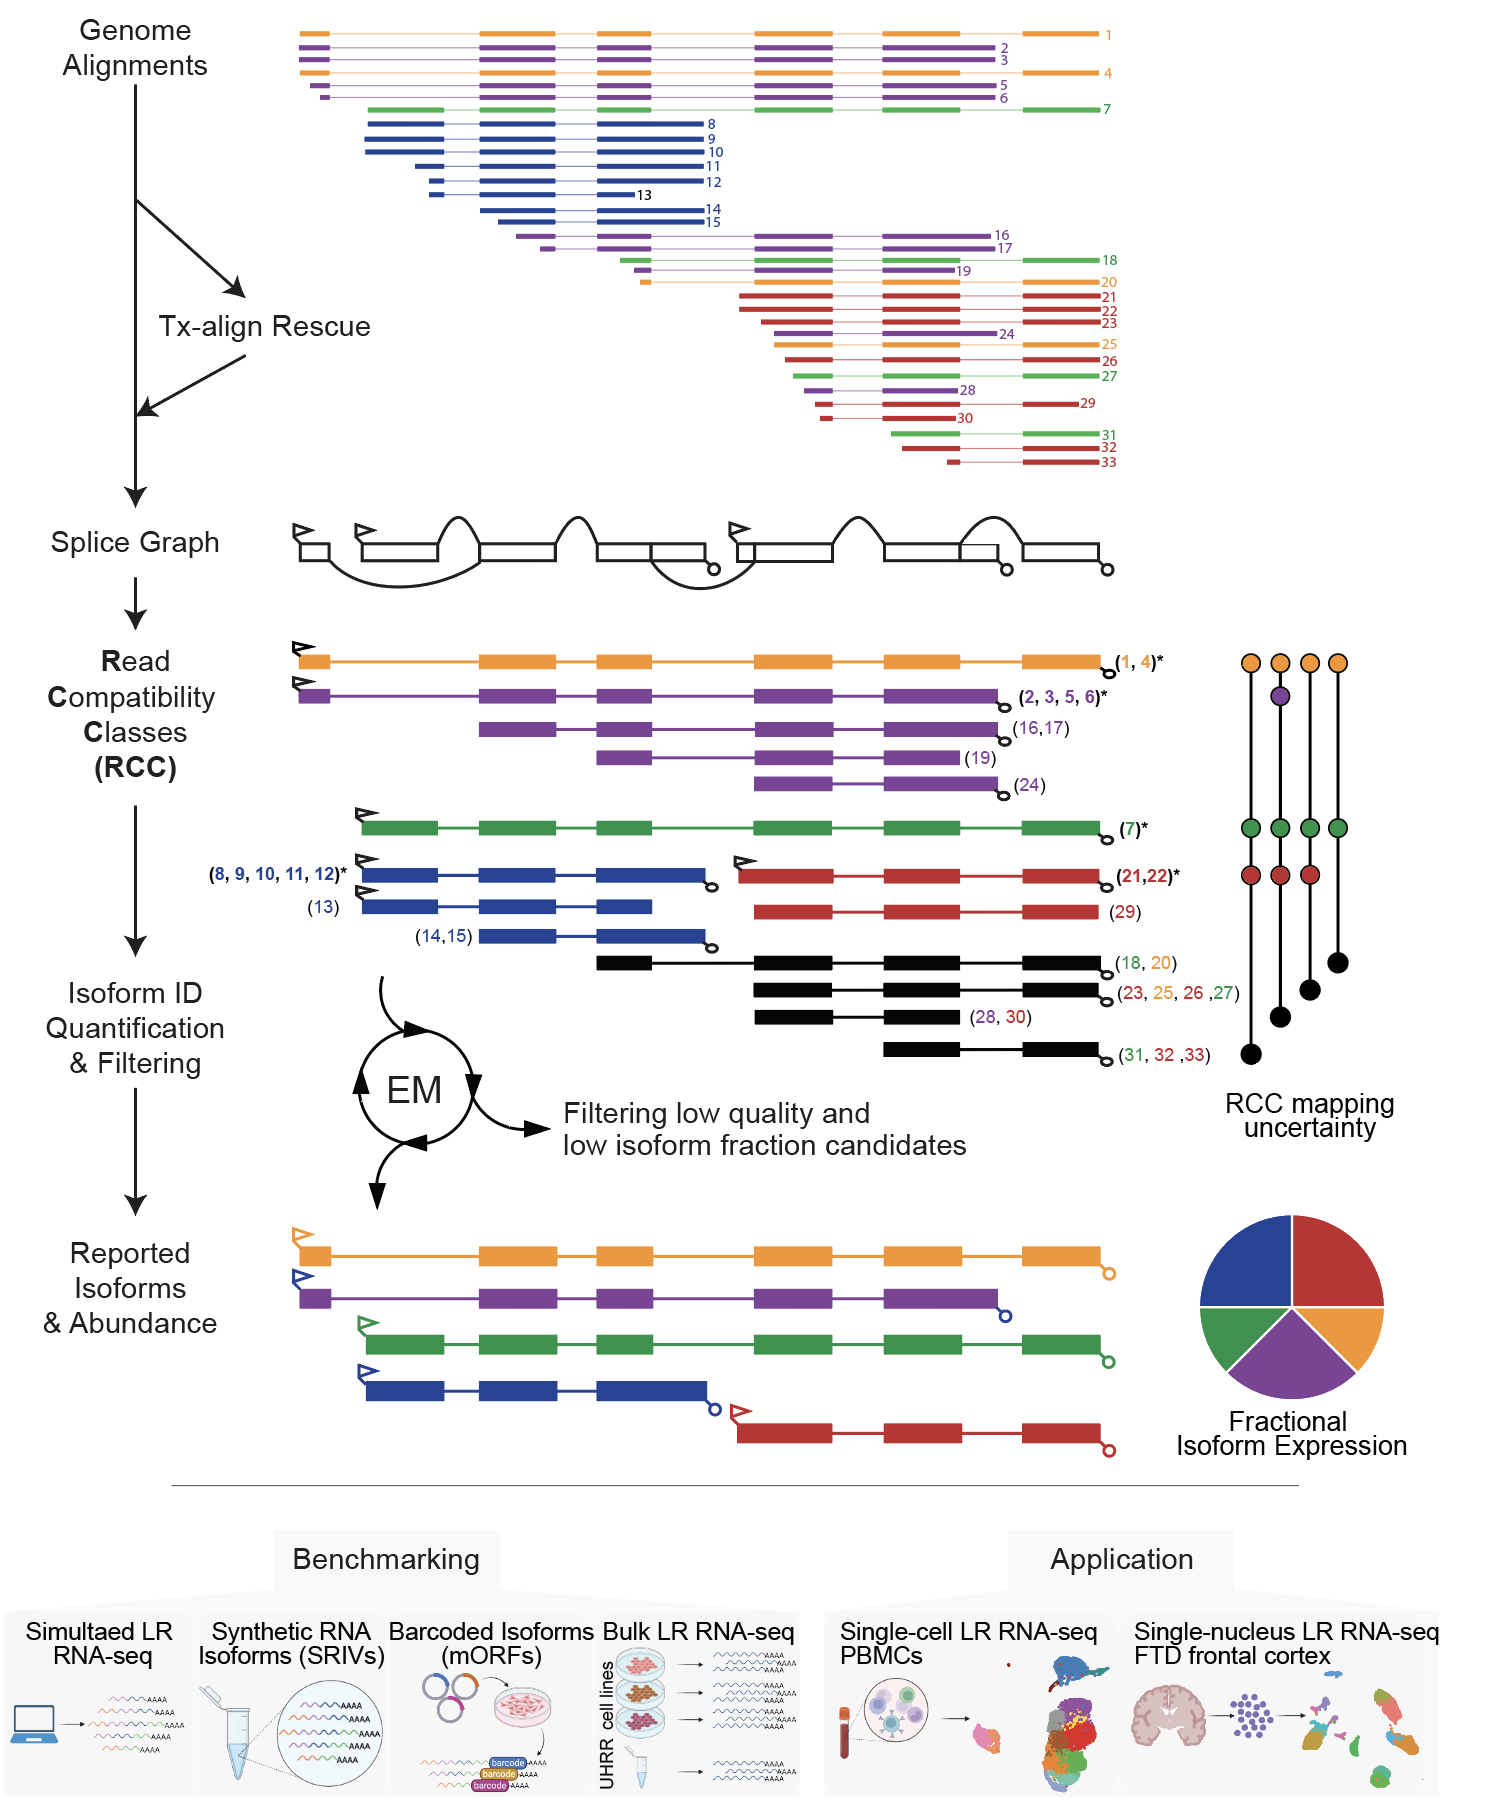
\includegraphics{figures/docx_export/Fig1.png}}
\end{center}

\captionof{figure}{\textbf{Conceptual overview of the LRAA algorithm for isoform identification and quantification in bulk and single-cell long-read transcriptomics.} A simplified overview of the LRAA workflow is shown, beginning with splice-aligned long-read isoform data and encompassing splice-graph construction, assignment of spliced read alignments or rescued direct-to-transcriptome (Tx-align) alignments to genome-based splice graph path nodes and grouping into read compatibility classes (RCC), assembly of candidate isoforms via compatible RCC collapse, and iterative quantification and filtering to define final isoform structures and abundance estimates. For illustrative purposes, read alignments are colored according to the isoforms from which they were derived and numbered to enable visual tracking through the splice graph and RCC relationships; in real RNA-seq data, the transcript of origin for each read is unknown a priori and must be fully inferred from alignment structures and compatibility relationships. Reads are numbered to allow tracking to the splice graph-based RCCs that they define. Top-level RCCs not compatible and contained by other RCCs are labeled with *. \doccomment{Houlin Yu}{2026-07-27}{Here, the sentence says "RCCs found compatible and contained by other top-level RCCs are colored black", my understanding is that here, RCCs are compatible with multiple other top-level RCCs.\\
Maybe I am missing something; If that is the case, I was thinking read 19 may also be black?}\doccomment{Houlin Yu}{2026-07-27}{Also read 29, are we missing a "polyA mark"?}\doccomment{Brian Haas}{2026-07-30}{good catch!~ I added " \textquotesingle splice-incompatible\textquotesingle{} RCCs" to differentiate the black ones.\\
Also, good catch with read 29. That exon should have been shorter than it is. Will update that in the fig.}RCCs found compatible and contained by other top-level splice-incompatible RCCs are colored black and the RCC mapping uncertainty matrix indicates the multiple compatibilities. RCCs with top-level RCC mapping uncertainty have read support fractionally assigned according to the EM. For clarity, several implementation details are abstracted in this schematic; a complete description of the algorithmic workflow is provided in \textbf{Supplementary Figure~\ref{sfig:1}}, which illustrates the construction of separate splice graphs for multi-exon and single-exon read alignments, their subsequent merging, and the downstream quantification and filtering steps. In the schematic, 5′ pointed triangles denote candidate transcription start sites (TSS), and 3′ trailing lollipops denote candidate transcription end sites (TES) or sites of polyadenylation. The LRAA identified isoforms were leveraged for multiple benchmarking and applications as shown (bottom).\doccomment{Houlin Yu}{2026-07-27}{For consistency, RCC mapping uncertainty shall be "RCC Mapping Uncertainty" - the first letter of the word being capitalized}\doccomment{Houlin Yu}{2026-07-27}{Also, "Filtering low qua.." and "FTD frontal.." (not sure about these)}\doccomment{Houlin Yu}{2026-07-27}{mORF, the original cell paper uses all capital letters. MORF}}\label{fig:1}

\subsection{Benchmarking isoform identification and quantification accuracy and study design}\label{benchmarking-isoform-identification-and-quantification-accuracy-and-study-design}

Benchmarking long-read isoform identification and quantification methods is challenging because no single dataset simultaneously provides complete ground truth and the complexity of real biological data. Different benchmarking substrates therefore offer complementary advantages, with each addressing distinct aspects of the problem.

Simulated long-read datasets provide complete knowledge of the isoform from which each read was generated, enabling unambiguous evaluation of isoform identification and abundance estimation even when reads are partial or compatible with multiple isoforms. However, simulated data lack many features of real sequencing experiments, including heterogeneous degradation patterns and the full complexity of transcript processing observed in biological samples, while platform-specific error profiles are necessarily modeled rather than directly observed.

Conversely, genuine long-read RNA sequencing data capture the biological and technical complexity that isoform analysis methods are designed to address, including variable transcript boundaries, partial transcripts, and technology-specific error characteristics. These datasets are therefore essential for evaluating practical performance in biologically relevant settings, but they lack definitive isoform-level ground truth. In particular, it is generally not possible to determine with certainty which isoform a partial read originated from, nor to enumerate all true full-length transcript structures present in a complex sample.

Synthetic spike-in standards, such as SIRVs and Sequins, occupy an intermediate position. These controls consist of real sequence data with defined transcript structures, enabling assessment under controlled conditions. However, because individual reads are not barcoded, the transcript of origin for each read is not directly observable, and these molecules are not expressed within native cellular contexts, limiting their ability to capture biological processing and degradation.

To bridge these gaps, we propose a new benchmarking framework based on Multiplexed Overexpression of Regulatory Factors (MORFs), which provides biologically expressed, barcoded isoforms for which the transcript of origin is known for every sequenced read. MORFs combine key advantages of simulated and real datasets by enabling unambiguous read-level truth assignment while preserving endogenous transcription, degradation patterns, and sequencing error characteristics. This framework allows direct evaluation of isoform discovery, read assignment, and abundance estimation under conditions that closely resemble real experimental data.

Across these benchmarks, definitions of true positives, false positives, and false negatives necessarily depend on both the properties of the dataset and the execution mode being evaluated. For simulated and MORF-based benchmarks, isoform- and read-level truth is explicitly defined, enabling direct assessment of identification and quantification accuracy. In contrast, for genuine whole-transcriptome datasets lacking definitive ground truth, evaluation focuses on structure-based comparisons and quantitative concordance rather than absolute correctness. For reference-guided analyses, isoforms provided as input are excluded from discovery-based performance metrics to ensure that evaluation is restricted to transcripts unknown to the method a priori. Below, we apply all these benchmarking strategies to enable evaluation of isoform identification and quantification performance across the diverse data types and analytical modes.

\subsubsection{Benchmarking isoform identification and quantification accuracy using simulated and genuine PacBio and ONT long isoform reads and reference data sets}\label{benchmarking-isoform-identification-and-quantification-accuracy-using-simulated-and-genuine-pacbio-and-ont-long-isoform-reads-and-reference-data-sets}

To evaluate isoform identification and quantification performance across diverse experimental conditions, we benchmarked LRAA and related methods using PacBio and ONT long-read reference datasets analyzed in the following progression. We first examined simulated long-read datasets, which provide complete knowledge of transcript structures and read origins, enabling direct evaluation of isoform identification and abundance estimation under controlled error models. We next assessed performance using SIRV spike-in controls, consisting of real long-read sequencing data generated from defined transcript mixtures that capture platform-specific error characteristics while retaining known reference structures. Finally, we analyzed MORF datasets, which provide biologically expressed reference transcripts with read-level origin information through isoform barcoding.

\textbf{Simulated long RNA-seq at variable sequencing error}

We evaluated isoform identification and quantification accuracy using simulated long-read strand-specific RNA-seq datasets, which provide a complete and unambiguous ground truth and enable controlled assessment of the impact of sequencing error and read truncation on performance. Long-read data were simulated for mouse and \emph{Arabidopsis thaliana} transcriptomes with platform-specific 3' and 5' end variable truncation at error-free conditions and at increasing total error rates of 1.6\%, 5.0\%, and 8.5\%. Across all simulations and execution modes, LRAA consistently ranked among the top-performing methods for both quantification and isoform identification (\textbf{Figure~\ref{fig:2}, Supplementary Figure~\ref{sfig:2}}). In quantification-only mode, most methods performed well with few exceptions, and LRAA was consistently among the most accurate. For reference-guided and annotation-free isoform identification, LRAA consistently yielded highest overall accuracy (F1 score) across error profiles with the exception of simulated error-free reads where ESPRESSO outperformed all methods in annotation-free isoform discovery. Most methods demonstrated resilience to higher error rates except for ESPRESSO, which continued to perform well but with degraded performance at higher error rates, Mandalorion, and most notably for IsoSeq, which is specifically tuned to PacBio high fidelity (HiFi) reads (\textbf{Supplementary Figure~\ref{sfig:2}}). While informative for contrasting method performance on tractable inputs, simulated data are imperfect models of genuine sequencing data and do not substitute for benchmarking on real datasets.

\paragraph{Spike-In RNA Variants (SIRVs)}\label{spike-in-rna-variants-sirvs}

We next evaluated isoform identification and quantification accuracy using Spike-In RNA Variants (SIRVs), which provide a defined set of transcript structures and relative abundances while retaining real sequencing and alignment characteristics. We analyzed PacBio Kinnex sequencing data for the SIRV mixes E0, E1, and E2, spanning equimolar to highly skewed expression distributions (\url{https://www.lexogen.com/store/sirv-set1/}). Across all three execution modes, LRAA consistently ranked as a top-performing method (\textbf{Figure~\ref{fig:2}, Supplementary Figure~\ref{sfig:3}}), achieving the highest combined precision and recall, as measured by F1 score, in most reference-guided and annotation-free isoform-identification settings. In quantification-only mode, LRAA achieved high accuracy across all SIRV mixes, with other probabilistic approaches including Oarfish, Isosceles, ESPRESSO, and Bambu also performing strongly. For isoform identification, performance varied by execution mode and expression mix. LRAA exhibited top accuracy for ref-guided and de novo isoform identification except for the SIRV E2 mix where ESPRESSO showed marginally higher accuracy in the reference-guided and de novo E2 evaluation. Methods such as IsoSeq and TALON exhibited high sensitivity but lower precision, resulting in reduced overall accuracy. While SIRVs provide a useful intermediate benchmark, they remain synthetic constructs and do not fully reflect native cellular processing of transcripts, which motivated us to explore MORFs as benchmarks described below.

\paragraph{MORFs}\label{morfs}

To benchmark isoform identification and quantification using genuine biological transcripts with unambiguous ground truth, we leveraged the (MORF library \citep{joung2023}. This resource comprises 3,548 human transcription factor isoforms representing 1,836 genes, expressed as lentiviral clones and each containing a unique isoform-specific barcode embedded at the 3′ end of the transcript (\textbf{Supplementary Figure~\ref{sfig:4}a}). These barcodes enable definitive assignment of every sequenced read, including partial reads, to its isoform of origin, thereby overcoming a central limitation of synthetic spike-in controls and genuine transcriptome data. After expressing the MORF library in HEK293 cells, we sequenced it using PacBio Kinnex and ONT MinION. The PacBio dataset represented 2,913 expressed isoforms from 1,560 MORF genes, whereas the ONT dataset represented 2,892 isoforms from 1,553 genes. We used these datasets to evaluate isoform identification and quantification in quantification-only, reference-guided, and annotation-free de novo modes (\textbf{Figure~\ref{fig:2} and Supplementary Figure~\ref{sfig:4}b}). LRAA achieved the highest overall accuracy for both isoform identification and quantification, except for de novo isoform identification mode with ONT where LRAA performed nearly identically to StringTie and ESPRESSO marginally outperformed both. As observed for SIRVs, IsoSeq and TALON exhibited high recall but substantially lower precision, resulting in reduced overall accuracy. Altogether, MORFs provided a more biologically informed benchmark that revealed shifts in relative method performance compared with SIRVs, most notably for Mandalorion, while also confirming that a subset of methods, including LRAA, consistently ranked among the top performers.

\begin{center}
\pandocbounded{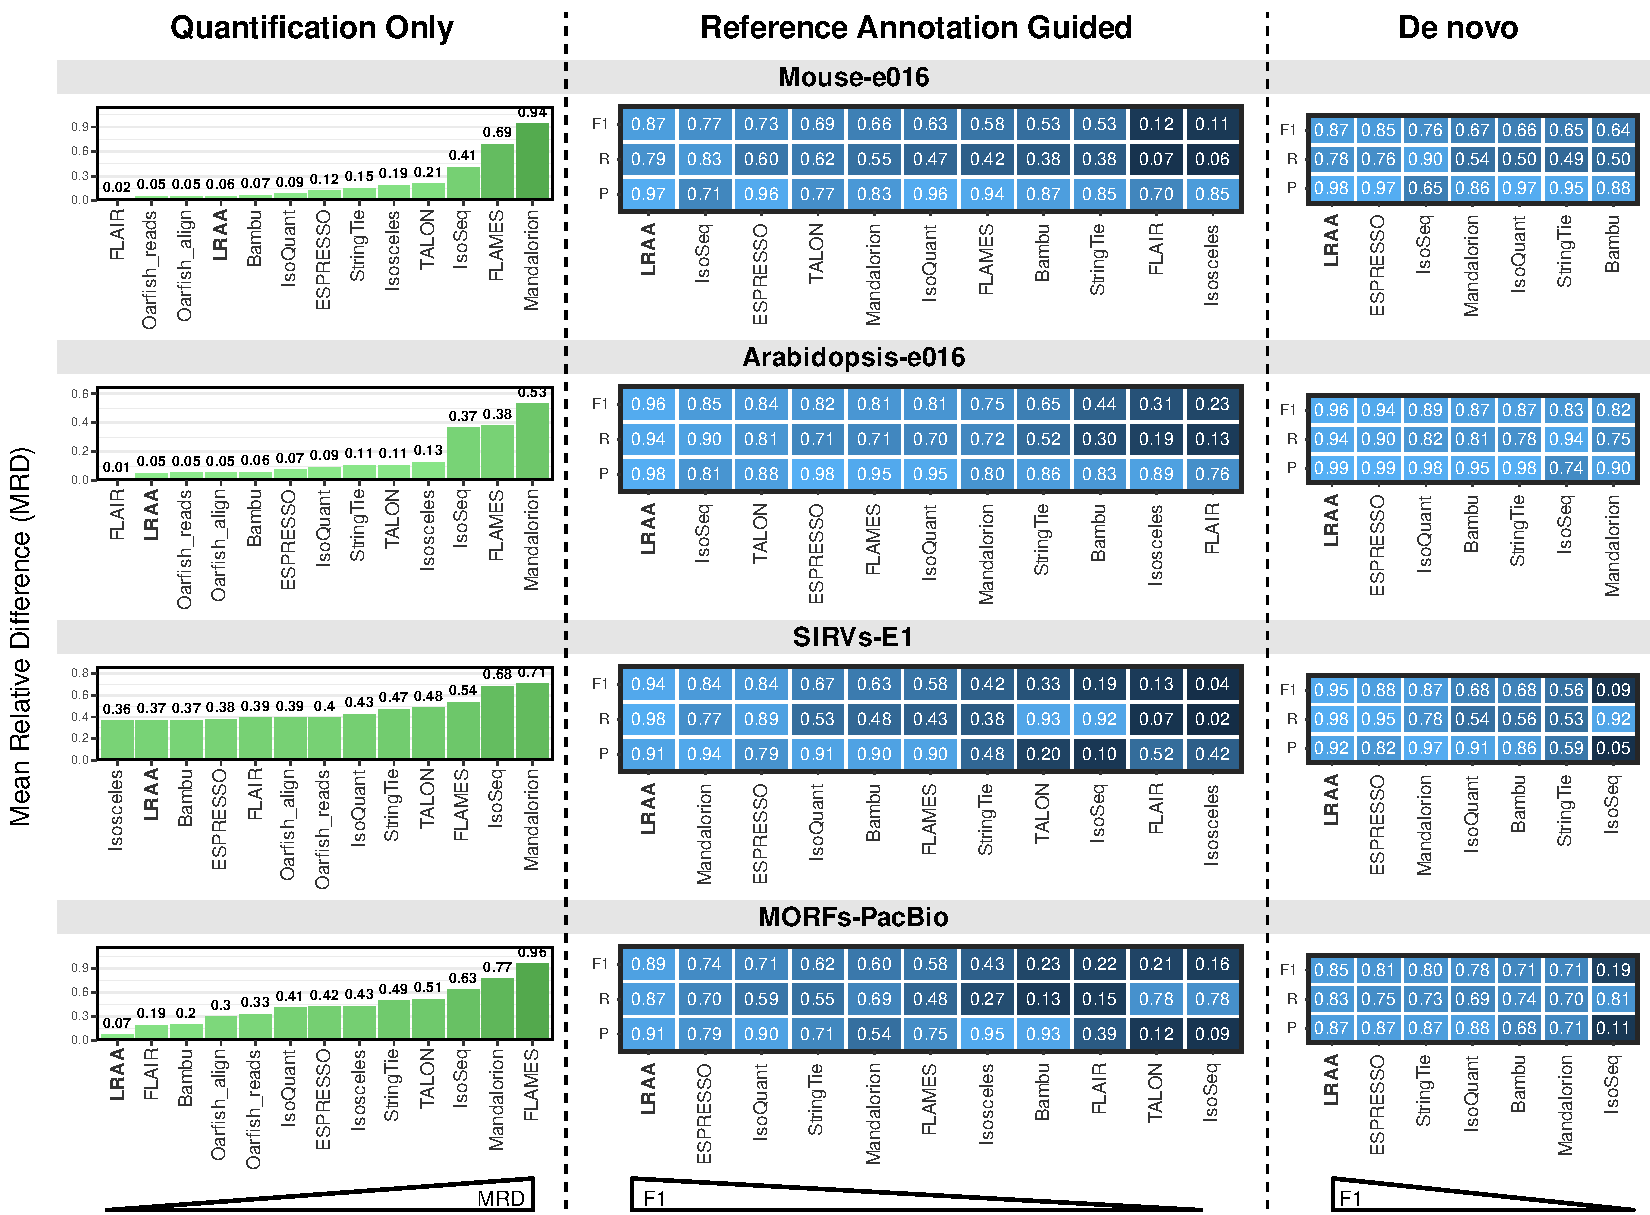
\includegraphics{figures/benchmark/Fig2_benchmarks_sims_SIRVs_MORFs.pdf}}
\end{center}

\captionof{figure}{\textbf{Isoform identification and quantification accuracy based on long read RNA-seq derived from simulated reads (Mouse and Arabidopsis) or genuine RNA-seq for sequencing standards}. Quantification (left column), reference annotation-guided isoform identification (center column), and reference annotation-free (de novo) isoform identification (right column) accuracies are indicated for evaluated methods based on the following data sets (top-to-bottom): simulated mouse and simulated Arabidopsis PacBio reads with 1.6\% error (e016 samples), and genuine PacBio Kinnex sequencing for SIRVs (E1 sample) and MORFs. Methods are ranked from left to right according to top accuracy based on mean relative difference for quantification and F1 score for isoform identification. See \textbf{Supplementary Figures~\ref{sfig:2}-4} for extended sample benchmarks for these targets.}\label{fig:2}

\paragraph{Whole transcriptome sequencing of cell lines and reference standards}\label{whole-transcriptome-sequencing-of-cell-lines-and-reference-standards}

While simulations, SIRVs, and MORFs enable benchmarking against defined truth sets, the primary use case for long-read isoform analysis methods is whole-transcriptome sequencing, where ground truth isoform structures and expression levels are not known. To evaluate performance in this setting, we analyzed bulk long-read transcriptomes generated using PacBio Kinnex for the BT474 and K562 cell lines, the lymphoblastoid sample GM24385 provided as Genome in a Bottle RNA reference sample for individual HG002 (\url{https://www.nist.gov/programs-projects/genome-bottle}), the Universal Human RNA Reference (UHRR) \citep{xu2014}, and Oxford Nanopore strand-specific cDNA sequencing for the A549 and MCF7 cell lines from the SG-NEx project \citep{chen2025}. Isoform identification accuracy was assessed using both reference-guided and annotation-free \emph{de novo} execution modes, with proxy truth sets defined based on agreement across methods and known reference annotations (see \textbf{Methods}). Across all PacBio Kinnex and both ONT datasets, LRAA ranked as the top-performing method for isoform identification in reference-guided execution mode. In de novo mode, ESPRESSO slightly outperformed LRAA on the PacBio Kinnex data sets to be top-ranked (\textbf{Figure~\ref{fig:3}}). In contrast, LRAA demonstrated highest accuracy on both ONT data sets and ESPRESSO was least accurate, suffering from especially low recall while retaining high precision (\textbf{Figure~\ref{fig:3}}).

Because no absolute expression ground truth is available for these datasets, we evaluated quantification consistency by comparing isoform-level expression profiles across methods using Pearson correlation. LRAA-derived expression profiles clustered closely with those from methods that performed best in quantification benchmarks with defined truth sets, including Oarfish, Isosceles, and Bambu. Overall, these results demonstrate that LRAA performs robustly across whole-transcriptome datasets and sequencing platforms, positioning LRAA as a highly effective approach for long-read transcriptome analysis.

\begin{center}
\pandocbounded{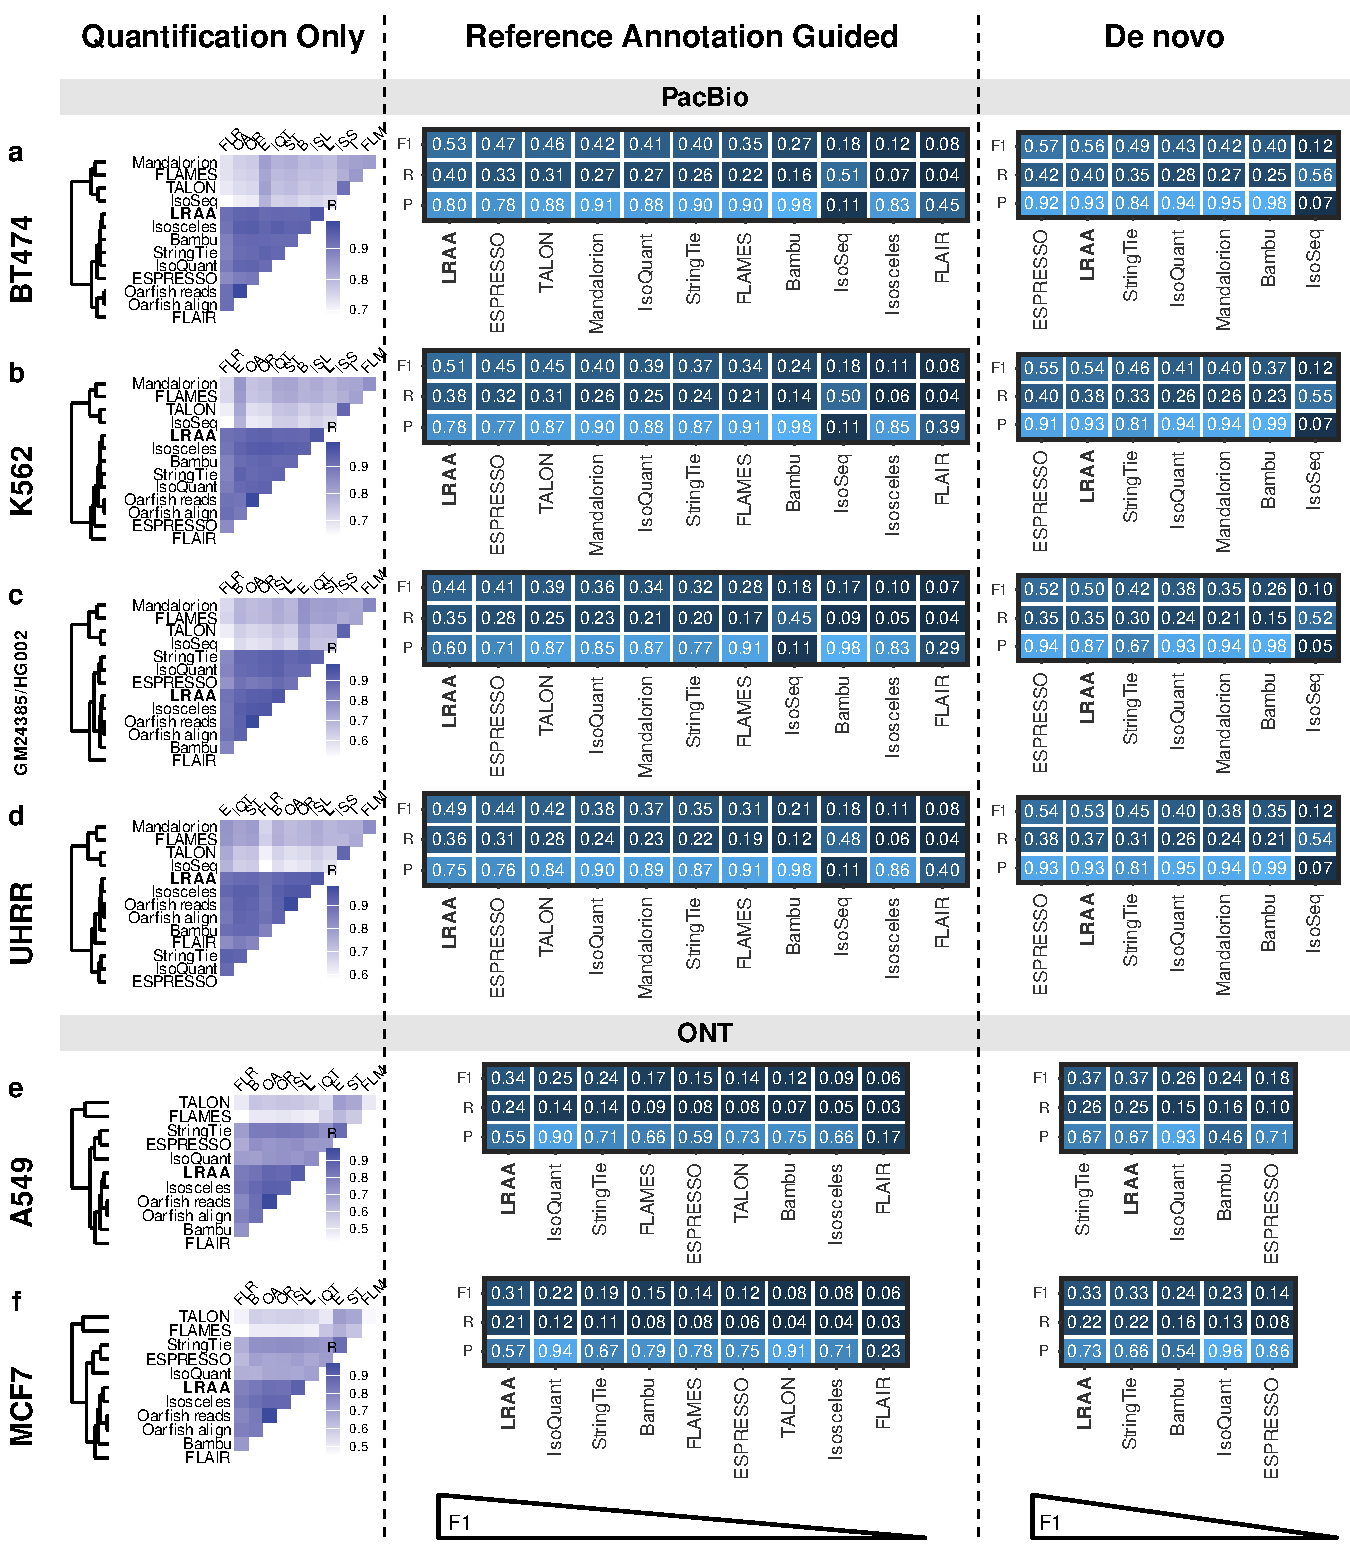
\includegraphics{figures/benchmark/Fig3_benchmarks_cell_lines.pdf}}
\end{center}

\captionof{figure}{\textbf{Benchmarking isoform identification and quantification accuracy using whole transcriptome sequencing of human cell lines and RNA reference samples.} Transcript quantification (left column), reference annotation-guided (center column) and reference annotation-free (de novo) isoform identification (right column) were evaluated for long read isoform analysis methods based on whole transcriptomes sequenced using PacBio Kinnex (top section) or ONT (bottom section). PacBio Kinnex sequenced transcriptomes correspond to (top-to-bottom) cell lines (a) BT474 and (b) K562 and (c) reference standards Genome In a Bottle RNA sample for GM24385/HG002 and (d) commercially available Universal Human RNA Reference (UHRR) from Thermo Fisher Scientific. ONT sequenced cell lines correspond to (top-to-bottom) (e) A549 and (f) MCF7. Expression quantification was evaluated by computing the Pearson correlations for isoform expression (log(TPM+1) values) and clustered by similarity. Isoform identification accuracy was estimated using proxy truth sets based on shared vs. uniquely identified isoforms (see \textbf{Methods}). Abbreviations used: FLR:FLAIR, B:Bambu, OA:Oarfish align, OR:Oarfish reads, L:LRAA, ISL:Isosceles, IQT:IsoQuant, E:ESPRESSO, ST:StringTie, FLM:FLAMES.\doccomment{Houlin Yu}{2026-07-27}{Bottom left MCF7 Quant plot: the labels of tools are a bit misaligned.}}\label{fig:3}

\subsubsection{Application of LRAA for de novo or reference-guided isoform identification in single-cell and single-nucleus long-read whole transcriptome sequencing.}\label{application-of-lraa-for-de-novo-or-reference-guided-isoform-identification-in-single-cell-and-single-nucleus-long-read-whole-transcriptome-sequencing.}

Application of long-read transcriptome sequencing at single-cell and single-nucleus resolution enables isoform-level analysis in heterogeneous tissues but introduces additional computational challenges relative to bulk data \citep{gupta2024, kumari2024, alkhafaji2024, hardwick2022}. In particular, individual cells contribute limited read depth, rare isoforms may be confined to specific cell populations, and single-nucleus data are enriched for partially processed transcripts. To address these challenges, we developed an LRAA single-cell workflow that integrates isoform identification and quantification with cell clustering, allowing isoform discovery to be informed by cell-type-specific expression patterns (\textbf{Figure~\ref{fig:4}}).

The LRAA single-cell workflow operates in two phases. In the first phase, LRAA is applied in pseudobulk mode to perform isoform identification and quantification using either reference-guided or annotation-free execution modes. Gene-level expression estimates derived from this phase can then be used to define cell clusters based on cell-barcoded read assignments or cluster assignments can be predefined by the user. In the second phase, isoform identification is performed separately within each cell cluster guided by the initial pseudobulk-based isoform structures, further enabling recovery of isoforms that are low abundance in the full pseudobulk but enriched within specific cell populations. Isoforms identified across clusters are subsequently merged into a unified isoform set, followed by a final round of cluster-aware quantification to generate gene-, isoform-, and splice-pattern-level expression matrices for downstream analysis.

We applied this workflow to two distinct long-read single-cell datasets generated using PacBio Kinnex sequencing of 10x 3′ libraries: peripheral blood mononuclear cells (PBMCs), representing a well-characterized and transcriptionally diverse cell population, and single nuclei isolated from frontal cortex tissue of an FTD donor, representing a challenging setting dominated by intronic reads and incomplete transcript processing.

\begin{center}
\pandocbounded{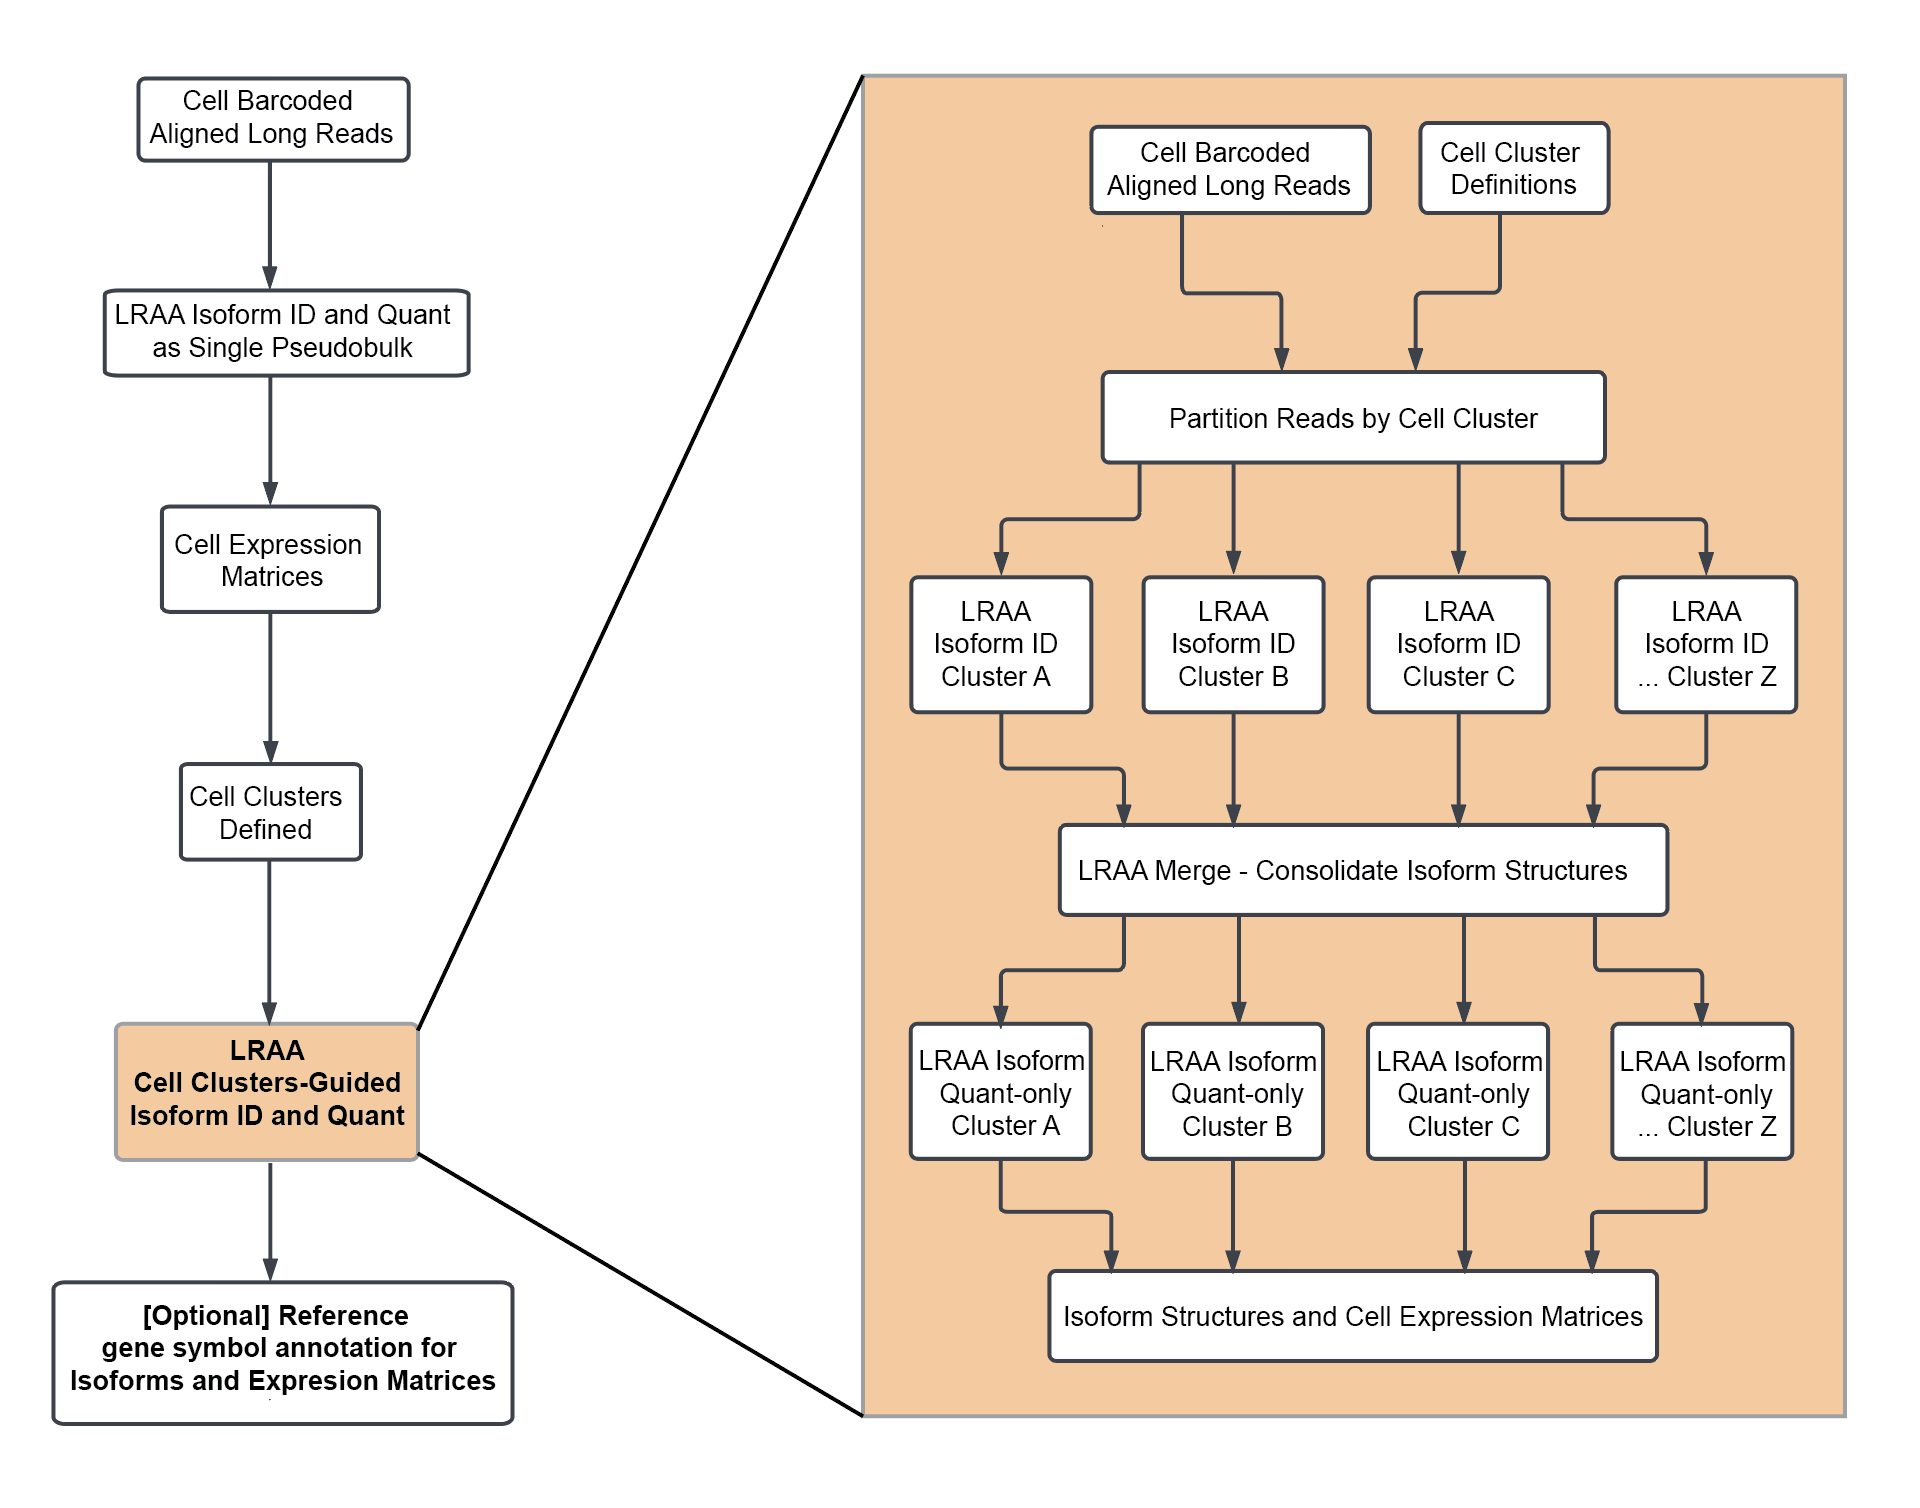
\includegraphics{figures/docx_export/Fig4.png}}
\end{center}

\captionof{figure}{\textbf{Pipeline for application of LRAA to single-cell transcriptomics data for novel isoform discovery.} LRAA is first leveraged for isoform identification and quantification in pseudobulk mode (yellow). Cell barcodes derived from isoform-assigned reads are leveraged to define cell clusters unless predefined as an input. LRAA is then used on a second phase where isoform identification is performed separately on each cell cluster, using the isoform structures defined in the initial phase for reference-guided isoform identification. The cell cluster-based isoforms are subsequently merged and unified followed by a final round of cell cluster-based quantification to assign reads (and cell barcodes) to the unified isoform set, ultimately retaining cell-type specific isoform structures.}\label{fig:4}

\paragraph{Isoform Detection via Single-Cell Kinnex from PBMCs}\label{isoform-detection-via-single-cell-kinnex-from-pbmcs}

We first applied the LRAA single-cell workflow to a PBMC sc-Kinnex dataset generated using PacBio sequencing of a 10x 3′ library totaling 82M reads for 10k cells. We examined the characteristics of individual long-read alignments relative to the reference annotation using an LRAA SQANTI-like classification (see \textbf{Methods}). A substantial fraction of reads corresponded to fully spliced matches (FSM, 29\%) and incompletely spliced matches (ISM, 9\%), with additional reads mapping to intronic or antisense regions (\textbf{Figure~\ref{fig:5}a}).

LRAA was run in both annotation-free de novo and reference-guided modes. To ensure consistent downstream comparisons across pipeline execution modes, instead of using automated within-pipeline cell clustering, we provided predefined cell clusters as a pipeline input and the same cluster assignments were used for subsequent cluster-guided isoform identification and quantification in both execution modes (\textbf{Figure~\ref{fig:5}c}). We compared isoform structures obtained from the initial pseudobulk phase and the final cluster-guided phase of the workflow. The ref-guided and cell cluster-guided phase yielded modest increases in FSM isoforms (9\%) but substantially increased the number of ISM (67\%) and novel isoforms (123\%), while also contributing many more single-exon transcripts, most of which were localized within introns or oriented antisense to annotated transcripts (\textbf{Figure~\ref{fig:5}b}).

Notably, the cluster-guided phase enabled recovery of isoforms that were present at low fractional abundance in the pseudobulk analysis but became prominent within specific cell clusters. Many such isoforms failed to meet minimum isoform fraction thresholds in the initial phase but exceeded these thresholds when evaluated within cluster-specific contexts (\textbf{Figure~\ref{fig:5}d}). Reference-guided execution increased the number of FSM isoforms relative to annotation-free discovery but had limited impact on the recovery of ISM and novel isoforms.

Using the reference-guided, cluster-guided isoform set, we examined differential transcript usage across PBMC cell clusters. We identified genes exhibiting shifts in dominant isoform usage driven by alternative splicing (mean 167 genes per pair of cell clusters), as well as genes with identical splice patterns but alternative transcription start or end site usage (mean 73 genes per pair cell clusters) (\textbf{Figure~\ref{fig:5}e}). Representative examples include isoform switching of \emph{AIF1} between non-classical monocytes and subsets of T cells, and alternative transcription start site usage of \emph{EMP3} across monocytes, dendritic cells, B cells, and T cell populations (\textbf{Figure~\ref{fig:5}f--p}).

To further characterize the functional implications of alternative isoform usage, we examined the protein structural differences between the two proteoforms encoded by alternatively used \emph{AIF1} isoforms across PBMC cell types (\textbf{Figure~\ref{fig:5}k}). Structural modeling revealed that AIF1\^{}6633d encodes a truncated protein containing only a partial EF-hand calcium-binding domain, while AIF1\^{}a9489 encodes the full-length protein with a complete EF-hand domain (\textbf{Figure~\ref{fig:5}k}). Superimposition of the two structures showed extensive overlap, with AIF1\^{}a9489 containing additional structured and unstructured regions that may confer distinct calcium-binding properties and protein-protein interaction capabilities. Both proteoforms matched known reference annotations in GENCODE v47, demonstrating that reference-annotated alternative splicing can generate proteoforms with substantially different structural and potentially functional properties.

These findings motivated us to systematically investigate the landscape of novel proteoforms, those arising from unannotated splice junctions or intron retention events, that may expand proteomic diversity beyond the reference annotation. To identify novel proteoforms in human PBMCs, we applied our classification pipeline to complete ORF protein sequences at three length thresholds (≥50 AA, ≥100 AA, ≥200 AA). At the ≥50 AA threshold, 80,661 unique proteins were detected, with novel proteoforms representing 13.4\% (10,844) of the total proteome (\textbf{Supplementary Figure~\ref{sfig:6}, top}). Notably, as stringency increased to ≥100 AA and ≥200 AA, the proportion of novel proteoforms remained more or less consistent at 14.0\% (8,365 of 59,923) and 12.6\% (4,572 of 36,325), respectively, indicating that novel splicing events generate proteoforms across the full spectrum of protein sizes. Analysis of novel proteoform composition revealed that novel splice junctions accounted for 81.8-85.2\% of novel proteoforms across all thresholds, while intron retention events contributed 14.2-17.6\%. A combination of both mechanisms accounted for 0.6-0.7\% of novel proteoforms. (\textbf{Supplementary Figure~\ref{sfig:6}, bottom}).

\begin{center}
\pandocbounded{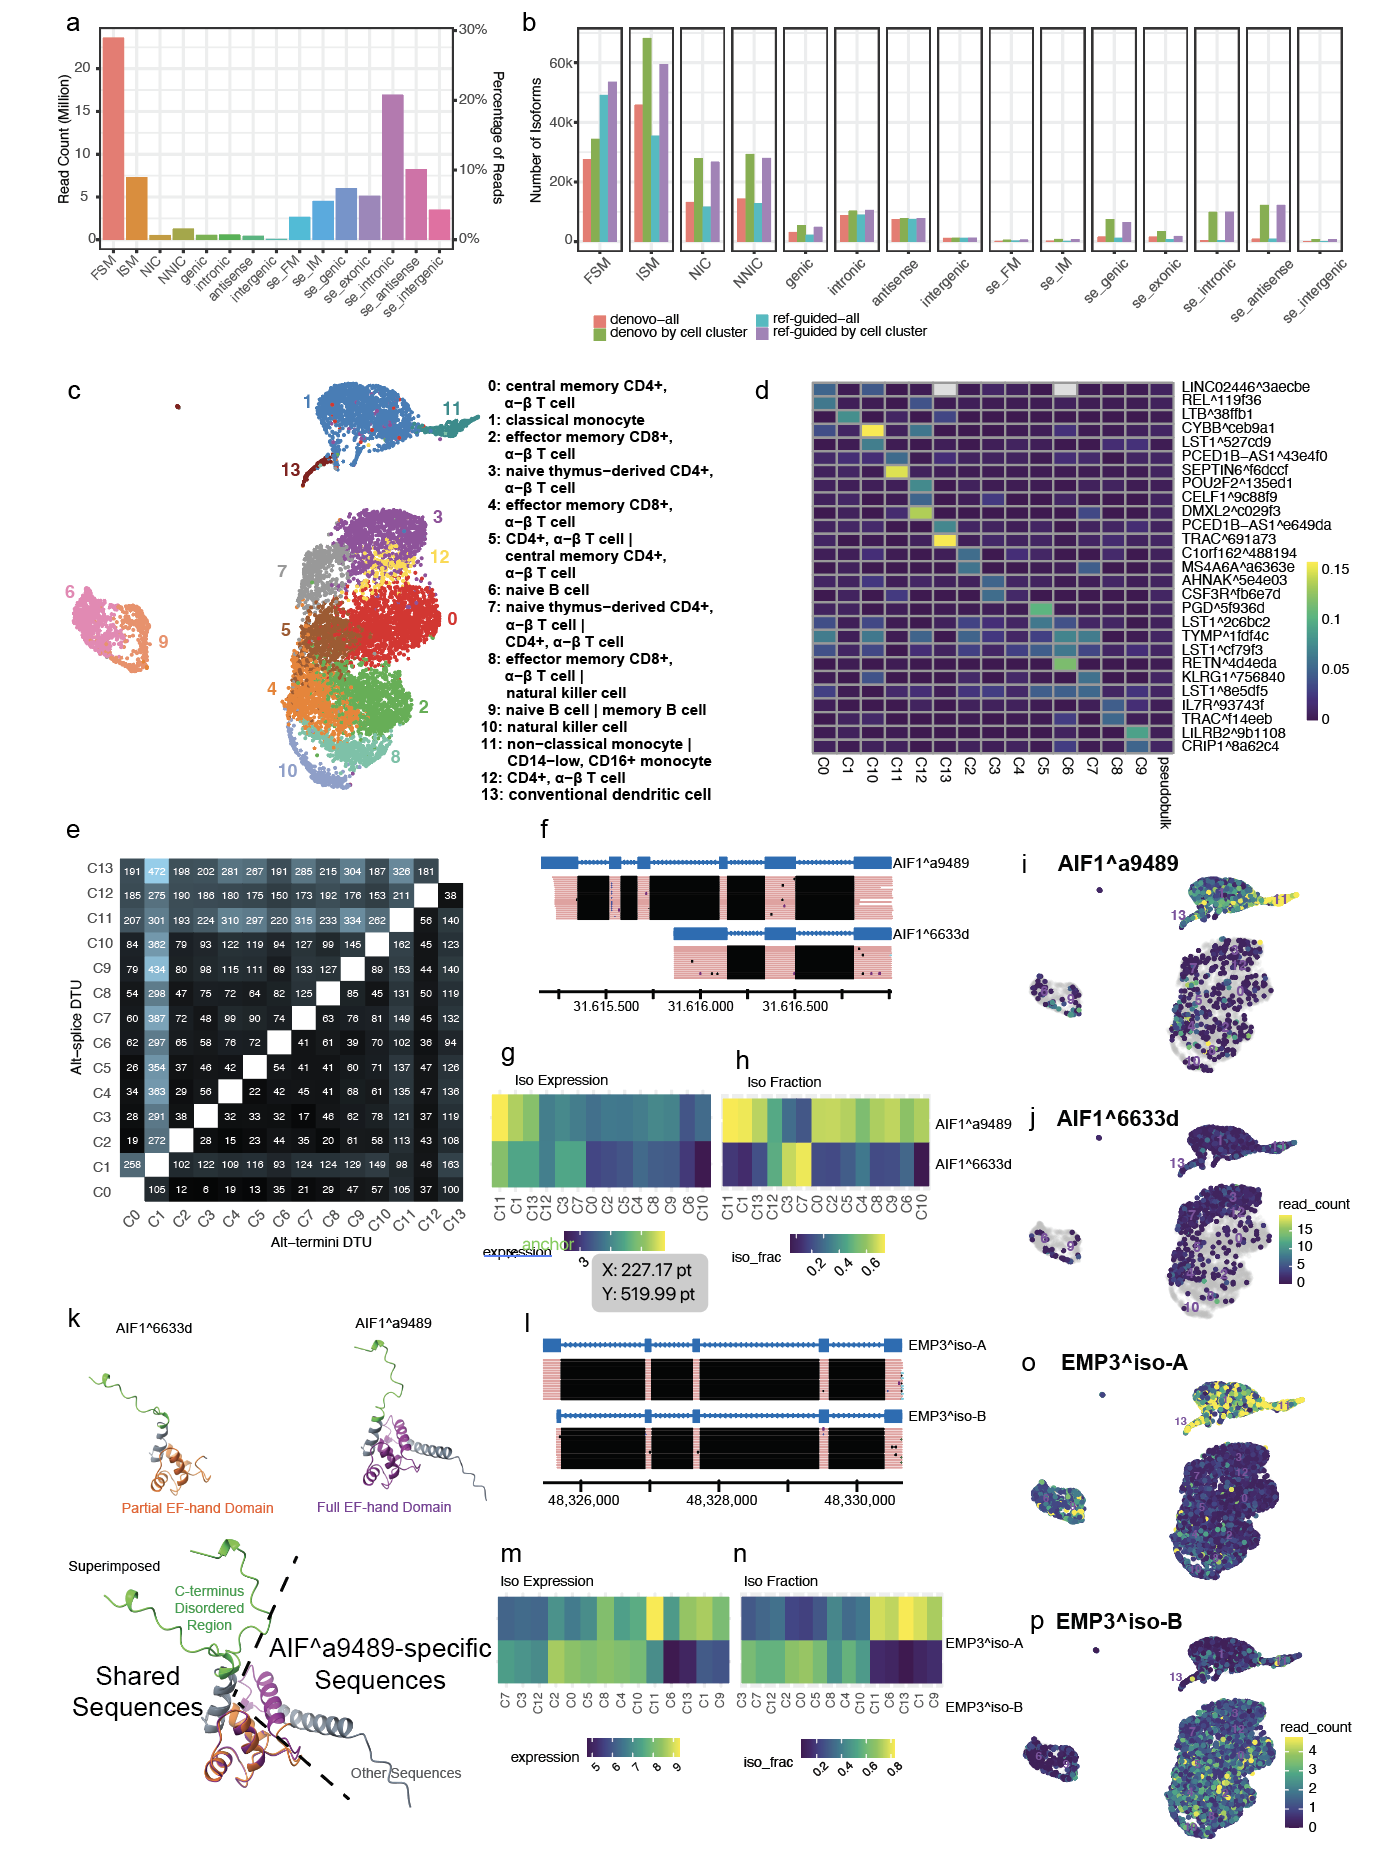
\includegraphics{figures/docx_export/Fig5.png}}
\end{center}

\captionof{figure}{\textbf{Isoform identification and quantification in PBMCs via LRAA with Kinnex scRNA-Seq.} (a) Counts and percentages of Kinnex reads assigned to gene structures or genome regions according to LRAA SQANTI-like categories. (b) Counts of LRAA-reconstructed isoforms from reference annotation-free (de novo) or reference annotation-guided workflows assigned to SQANTI-like categories. Isoforms with identical splice patterns but different termini boundaries are counted non-redundantly as collapsed. (c) UMAP for PBMCs based on LRAA-derived gene expression in quantification-only mode with dominant inferred cell types indicated. (d) Examples of isoforms estimated to have \textless1\% isoform fraction in pseudobulk mode but ≥ 5\% isoform fraction in at least one cell cluster context. (e) Counts of genes with detected differential transcript usage (DTU, upper triangle) or having identical splicing patterns but alternative termini usage (ATU, lower triangle) by cell cluster comparison. (f-j) DTU detected for two isoforms of the AIF1 gene with (f) isoform structures and supporting full-length Kinnex reads, (g) isoform expression, (h) isoform fraction, and (i,j) cellular expression shown for each isoform. (k) Structural modeling of AIF1 proteoforms. (l-p) ATU in the form of alternative transcriptional start sites detected for two isoforms of the EMP3 gene with (l) isoform structures and supporting full-length Kinnex reads, (m) isoform expression, (n) isoform fraction, and (o,p) cellular expression shown for each isoform.\doccomment{Houlin Yu}{2026-07-27}{5g, bottom, we have some unwanted elements}\doccomment{Houlin Yu}{2026-07-27}{m and n, right side, the isofrom ids are misaligned}}\label{fig:5}

\paragraph{Isoform Detection in Single-Cell Nuclei from an FTD Brain Frontal Cortex Sample}\label{isoform-detection-in-single-cell-nuclei-from-an-ftd-brain-frontal-cortex-sample}

We next applied the LRAA single-cell workflow to long-read single-nucleus RNA-seq data generated from frontal cortex tissue of an FTD donor. Single-nucleus sequencing enables transcriptional profiling of cell types that are difficult to capture using whole-cell approaches, but the resulting data are enriched for unspliced and partially processed transcripts, posing challenges for isoform-level analysis.

The FTD frontal cortex dataset was generated using PacBio Kinnex sequencing of a 10x 3′ single-nucleus library, yielding approximately 55 million long reads for 6.5k nuclei. In contrast to the PBMC sc-Kinnex data, the largest fraction of reads was classified as intronic (42\%), combining both intronic categories in the LRAA SQANTI-like read classification, with substantially fewer reads corresponding to fully spliced matches (3\%) or incompletely spliced matches (4\%) (\textbf{Figure~\ref{fig:6}a}). Despite this, LRAA identified large numbers of isoforms in both annotation-free and reference-guided execution modes; in the initial pseudobulk phase, reference-guided analysis yielded approximately three times as many fully spliced isoforms as annotation-free analysis (\textbf{Figure~\ref{fig:6}b}). For cluster-guided isoform identification, we similarly provided predefined cell clusters as input to the pipeline to enable consistent comparisons across clusters.

Comparison of the initial pseudobulk phase and the cluster-guided phase showed limited differences in the number of fully spliced matched isoforms, but substantial increases in incompletely spliced matched (25\% increase for de novo and 55\% increase for reference-guided) and novel isoforms (37\% increase for de novo and 56\% increase for reference-guided) following cluster-guided isoform discovery (\textbf{Figure~\ref{fig:6}b}). The abundance of intronic reads did not lead to a proportional increase in intronic isoform calls, consistent with LRAA\textquotesingle s stringent filtering based on read support, transcription start site evidence, and transcript end site evidence.

Gene-level expression profiles derived from the quantification-only phase were used to identify 14 distinct cell clusters corresponding to major brain cell types, including excitatory and inhibitory neurons, astrocytes, oligodendrocytes, microglia, endothelial cells, and fibroblasts (\textbf{Figure~\ref{fig:6}c,d}). Several of these cell types were further resolved into transcriptionally distinct subpopulations, often differing substantially in the number of expressed genes per nucleus (\textbf{Figure~\ref{fig:6}d}). Pairwise differential expression analysis between paired cell type subpopulations coupled with functional enrichment analysis indicated one subpopulation to be generally more active than the other coupled with stress responses. We refer to these as active or quiescent subpopulations below.

Using the reference-guided, cluster-guided isoform set, we examined differential transcript usage across cell clusters. Despite the predominance of intronic reads, we identified genes exhibiting significant shifts in isoform usage between cell types (\textbf{Figure~\ref{fig:6}e}). Among these, we detected the pathogenic cryptically spliced isoform of \emph{STMN2}, a hallmark of TDP-43 proteinopathy in FTD (\textbf{Figure~\ref{fig:6}f--j}) \citep{prudencio2020, melamed2019, klim2019}. Expression of \emph{STMN2} transcripts was most prevalent in excitatory neuron clusters 8 and 1, where \emph{STMN2} expression was detected in 40\% and 37\% of nuclei, respectively. However, the fraction of nuclei expressing the cryptically spliced isoform differed substantially between these clusters, with 18\% of active cluster 8 nuclei showing evidence of the cryptic isoform compared to 9\% in quiescent cluster 1. Inhibitory neuron clusters (active) 4 and (quiescent) 6 also exhibited \emph{STMN2} expression in 18\% and 10\% of nuclei, respectively, but the cryptically spliced isoform was detected in only 2\% and 1\% of nuclei in these clusters.

In addition to alternative splice pattern usage, we identified cases of alternative transcript end site usage without changes in splice structure. One such example involved \emph{EIF1}, where isoforms with identical splicing patterns but distinct polyadenylation sites were detected across multiple cell types, with the most pronounced shifts observed between oligodendrocytes and endothelial cells (\textbf{Figure~\ref{fig:6}k--o}).

We applied the same proteoform analysis pipeline to FTD brain frontal cortex samples. Novel proteoforms represented 5.5\% (3,639 of 66,109), 5.9\% (2,775 of 46,967), and 5.0\% (1,403 of 27,998) of the total proteome at ≥50 AA, ≥100 AA, and ≥200 AA thresholds, respectively (\textbf{Supplementary Figure~\ref{sfig:7}}). Consistent with PBMC samples, novel junctions predominated across all thresholds (65.6-72.9\%), while intron retention contributed 26.5-33.9\%. A combination of both mechanisms accounted for 0.5-0.6\% of novel proteoforms.

\begin{center}
\pandocbounded{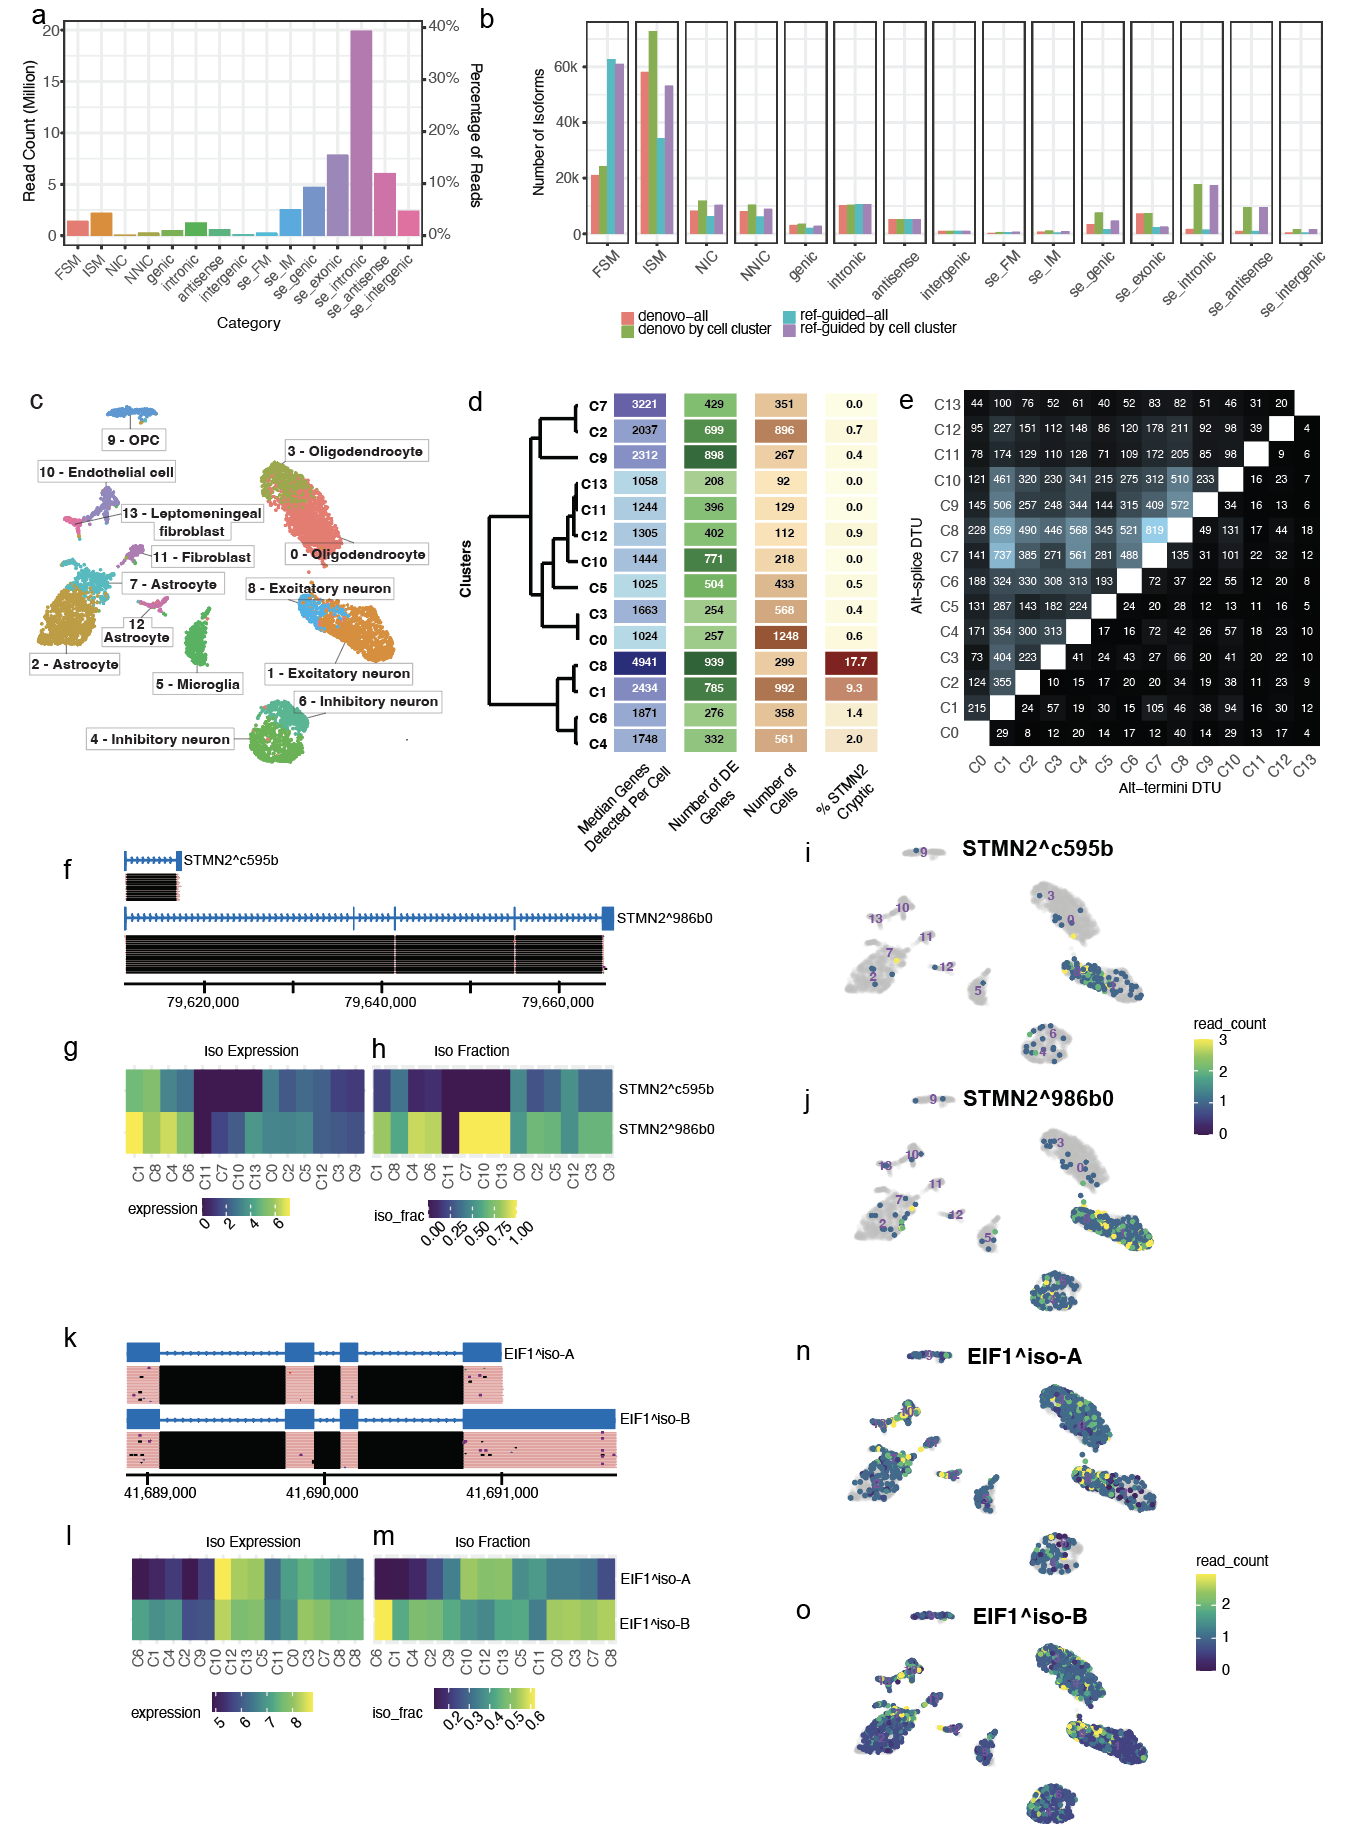
\includegraphics{figures/docx_export/Fig6.png}}
\end{center}

\captionof{figure}{Isoform identification and quantification in an FTD brain frontal cortex via LRAA with Kinnex snRNA-Seq. (a) Counts and percentages of Kinnex reads assigned to gene structures or genome regions according to LRAA SQANTI-like categories. (b) Counts of LRAA-reconstructed isoforms from reference annotation-free (de novo) or reference annotation-guided workflows assigned to SQANTI-like categories. (c) UMAP for FTD frontal cortex sample based on LRAA-derived gene expression in quantification-only mode with dominant inferred cell types indicated. (d) Overview of cell cluster properties and dendrogram showing relationships between cell clusters based on numbers of differentially expressed genes defined as cluster-specific biomarkers \doccomment{Houlin Yu}{2026-07-27}{Do we need these~details here?}\doccomment{Houlin Yu}{2026-07-30}{@bhaas@broadinstitute.org~ will double-check style and whether we need}(p\_val\_adj \textless{} 1e-5 \& abs(avg\_log2FC) \textgreater= 2). (e) Counts of genes with detected differential transcript usage (DTU, upper triangle) or having identical splicing patterns but alternative termini usage (ATU, lower triangle) by cell nuclei cluster comparison. (f-j) DTU detected for two isoforms of the \emph{STMN2} gene with (f) isoform structures and supporting full-length Kinnex reads, with the pathogenic cryptic isoform at top and canonical \emph{STMN2} isoform at bottom, (g) isoform expression, (h) isoform fraction, and (i,j) cellular expression shown for each isoform. (k-o) ATU in the form of alternative polyadenylation sites detected for two isoforms of the \emph{EIF1} gene with (k) isoform structures and full-length Kinnex reads, (l) isoform expression, (m) isoform fraction, and (n,o) cellular nuclei expression shown for each isoform.}\label{fig:6}
